\documentclass[pageno]{jpaper}
\newcommand{\IWreport}{2012}
\usepackage[normalem]{ulem}
\usepackage{setspace}

\begin{document}

\title{Holograsp: Bringing Virtual Objects into the Real World for Natural 3D Manipulation}

\date{}
\author{Edward Zhang}
\maketitle
%\doublespacing
\onehalfspace
\thispagestyle{empty}

\begin{abstract}
Traditional computer interfaces, namely the mouse and monitor, are inherently 2D. Thus, performing 3D tasks using
these interfaces is often challenging because both input and output are missing a dimension. Surprisingly,
previous work has consistently found the mouse to be superior to custom devices with three or more degrees
of freedom (DOF). We hypothesize that the disconnect between the input device and the visual feedback is the
source of the poor performance of high DOF devices. To investigate this hypothesis, we developed the Holograsp
system. Holograsp uses a stereoscopic 3D monitor to display virtual 3D objects as if they were floating in
space in front of the monitor; users can reach out and grasp these models to move them, as if they were real
objects. We performed an experiment comparing the efficacy of Holograsp with traditional 2D input and output
interfaces by measuring the time taken to complete 3D placement tasks. The results show that, although the
pop-out stereoscopic effects were difficult for some people to perceive, the combination of stereoscopic 3D
feedback and natural gestural interface was by far the most effective and intuitive system.
\end{abstract}

\newpage
\tableofcontents
\newpage

\section{Introduction}

In this paper we make two main contributions:
\begin{itemize}
\item We present Holograsp, a 3D manipulation system, to show the feasibility of colocating display and gestural spaces.
\item We show the benefits of such systems through a user study involving 3D manipulation tasks, in which we compare the
performance of Holograsp with traditional interfaces.
\end{itemize}

% ------------------------------------- RELATED WORK ----------------------------------------
\section{Background and Related Work}
\subsection{Mixed Reality}
Effective usage of computer systems depends on how users conceptualize their interactions with the system.
Perhaps the most obvious method is to present computer data in a physically motivated setting, translating
human intuition about the physical world into natural interactions with the system. Because of the nature of 3D data,
it is especially appropriate to conceptualize 3D interactions in physical terms. Milgram and Kishino present
the virtuality continuum of {\bf Mixed Reality} environments, describing the degree of overlap between the
real world environment and the system's virtual environment, in \cite{milgram1994taxonomy}. Real environments, namely
the real world, contain only real objects, and {\bf Virtual Reality} environments, such as 3D worlds in video games, contain only
virtual objects. A well-known intermediate between these two extremes is {\bf Augmented Reality}, in which virtual
objects are placed within the real world. such as the CAD modelling systems in the Iron Man films. Another intermediate is
{\bf Augmented Virtuality}, in which some real objects (usually the user's own body) are placed within a virtual world; a common
example of augmented virtuality is green-screening, where a user interacts in front of a blank screen but is displayed in a
different, virtual world.

\subsection{Virtual Reality}
There has been a significant amount of academic work published on virtual reality, especially
in {\bf immersive virtual reality}, where the user perceives themselves to be in the virtual environment. Immersive
virtual reality systems generally use Head-Mounted Displays (HMDs) for complete visual immersion, and have been studied
as far back as 1968, when Sutherland introduced the first HMD \cite{sutherland1968head}. Although immersive virtual reality
systems provide perceptual realism, interaction with such systems is difficult because users cannot physically see any input devices.
Some systems have the human body as the main interface controller, such as \cite{laviola1999whole, laviola1999flex}. Other systems render
virtual analogues of physical input devices, such as the virtual tablet in \cite{poupyrev1998virtual} or the cubes used in \cite{mine1997exploiting}.
Another common strategy is to use multimodal input, especially the combination of physical and voice systems, as in \cite{bolt1980put}.
In all of these cases, the visual feedback is critical for effective usage of these devices.

\subsection{Augmented Reality}
In contrast to virtual reality, {\bf Augmented Reality} involves placing virtual objects within the real world. The main challenge
in augmented reality is placing virtual objects into the real world. This involves two components: displaying the object, and
determining the location of the virtual object relative to the display \cite{zhou2008trends}. Although early systems focused on head mounted displays,
many drawbacks such as latency, field of view, and improper tracking \cite{hoffman2008vergence} have resulted in a shift towards different display methods.
Commercial and academic augmented reality systems now tend to use smartphones and tablets as "windows" into the augmented world. In this usage, the device's camera
image is combined with virtual objects to be displayed on the screen, so that moving the "window" around presents different views of the real environment; such systems
include DRIVE \cite{kim2011drive} and T(ether) \footnote{http://kiwi.media.mit.edu/tether/}.

Another aspect of augmented reality is tracking of a display's location so that the virtual object can be correctly overlaid onto the display.
Currently, the dominant strategy for tracking is to use fiducial markers. Fiducial markers are two-dimensional shapes placed in the environment
that can be used to determine the relative position and orientation of a camera using computer vision techniques. Works using fiducial markers include
\cite{kato1999marker, artoolkit, dedual2011creating}. Newer methods based on fiducial tracking can use arbitrary 2D images or structures as markers \cite{ferrari2001markerless, simon2000markerless}.
Note that these marker-based techniques do not function
well if the markers are blurred, partially occluded, out of view, inconsistently lighted, or at extreme angles; some of these challenges are investigated in \cite{fiala2010designing}. Other methods of tracking include inertial
tracking, which use accelerometers and gyroscopes without an external frame of reference \cite{lang2002inertial}, and markerless tracking, which uses optical flow and
stereo reconstruction techniques to determine 3D motion of the camera \cite{comport2006real}.

\subsection{Colocation of Hands and Virtual Manipulation Controllers}
Although several 3D manipulation systems have direct mappings between hand position and a virtual hand, such as \cite{poupyrev1996go},
comparatively few aim to make the perceived 3D position of the hand proxy be coincident with the user's natural perception of their
hand location. The relevant perceptual phenomenon, known as {\bf proprioception}, is a person's automatic knowledge of the position and orientation of their
limbs relative to themselves. The use of proprioception in 3D interfaces was heavily investigated by Mine in \cite{mine1997exploiting}, which found that
in an immersive virtual environment, manipulating objects colocated with the users hand was more efficient than manipulation at an offset. Several systems,
such as \cite{mulder2002personal, prachyabrued2011dropping}, use a tabletop with a mirrored display above it; in these systems the interaction space underneath
the display is directly mapped to what the user sees in the display. The preceding systems are strictly virtual reality systems, since the actual environment displayed
is still completely synthesized. Recent work by Microsoft Research, such as the Holodesk \cite{holodesk}, has instead used half-silvered mirrors to create an augmented reality
interaction space, where the user can see their hands interacting with colocated virtual objects. Holodesk focused on realistic physical interactions within the space,
representing real objects as point clouds that could knock over or hold up other objects. As far as we are aware, the Holodesk is the only existing system to augment a real
interactive space with colocated virtual objects.

\subsection{Evaluation of 3D User Interfaces}
Several studies have investigated the effectiveness of novel, high-DOF input devices by directly comparing them to traditional devices, especially the mouse.
Evaluation methods generally involve performing fundamental 3D tasks, especially selection, placement, and rotation. Input methods are compared based on their
speed and accuracy. The SpaceNavigator, a commercially available high DOF devices, was found to be inferior to the mouse for placement tasks in
\cite{mattheiss2011navigating}. B{\'e}rard et al also found the mouse to be more effective than several high-DOF devices for placement tasks
in \cite{study1}.  However, a later study by the same group found that enhanced visual feedback, in the form of pop-up depth views, greatly enhanced the effectiveness
of the high-DOF device, and was found to perform better than the mouse \cite{study2}. The
evaluation of the Holodesk system also involved a user study, in which they compared performance on a selection task with varying depth cues. They found that aligned
stereoscopic display systems were better than aligned non-stereoscopic systems with appropriate occlusion cues, and unaligned displays were slowest \cite{holodesk}.
We borrow our primary experimental procedure from \cite{study1, study2}.
% ------------------------------------- IMPLEMENTATION --------------------------------------
\section{The Holograsp System}
\subsection{Overview}
%TODO
\subsection{Software Architecture}
Holograsp uses a heavily abstracted engine to facilitate substitution of input and output devices, client applications, and SDKs.
The architecture of the engine invites the construction of many client applications; Holograsp provides the alignment of the
gestural and display spaces while the client program is free to use the display and input in any way. Our example application
is the timed 3D manipulation task harness used in the experiments section. The incarnation of the architecture used in the
experiments used DirectX for graphics rendering, the Nvidia API for configuring the 3D monitor, and the Intel Perceptual
Computing SDK for input.
\subsubsection{Holograsp Engine}$ $\\
The core engine uses the SDL library \footnote{http://www.libsdl.org/} for fundamental windowing and event handling.
The engine performs the following tasks:
\begin{itemize}
\item Check for and handle mouse, keyboard, and application events.
\item Check for new data from gestural input devices.
\item Buffer and preprocess any new data into a standard form, specifically finger coordinates and depth maps.
\item Transform the raw data into application-specific data, such as parsing finger coordinates into a hand pose.
\item Call application specific update functions, such as translating and rotating objects or creating new models.
\item Render the scene in stereoscopic 3D.
\end{itemize}

Most of these tasks are delegated to their own handlers, which are often application-specific.

\subsection{Stereoscopic Display Hardware}
One of the core aspects of Holograsp is the stereoscopic 3D. There are two competing standards for stereoscopic 3D rendering for computers
that are tied to the main graphics card manufacturers, Nvidia and AMD. Nvidia's 3D Vision system \footnote{http://www.nvidia.com/object/3d-vision-main.html}
produces packaged hardware systems including high quality shutter glasses and wireless synchronization stations that are guaranteed to work with Nvidia
graphics cards and supported monitors; the AMD HD3D system does not provide a unified system \footnote{http://www.amd.com/us/products/technologies/amd-hd3d/Pages/hd3d.aspx}.

In our setup, we used an Nvidia GTX555 consumer graphics card with a 27 inch Acer VG278H 3D monitor. The standard Nvidia shutter glasses use infrared
signals to synchronize the shutters with the display; since all of the depth cameras we tested used infrared for depth information, this resulted in
unacceptable interference. To eliminate this interference, we used the shutter glasses and synchronization station from the Nvidia 3D Vision Pro
package, which uses radio frequencies for synchronization.

\subsection{Stereoscopic Rendering}
Nvidia's 3D Vision supports two methods of rendering in stereoscopic 3D. Quad-buffered stereo rendering allows developers to render the scene for each
eye separately in OpenGL, and provides maximal control of stereo effects. 3D Vision Automatic allows any application running using Direct3D to be
displayed in stereoscopic 3D, without any additional development overhead \cite{nvidia3dvision}. Quad-buffered stereo is only supported on higher-end
professional graphics cards, whereas 3D Vision Automatic is supported on all newer Nvidia graphics cards. Therefore, we elected to use 3D Vision Automatic
for stereoscopic display.

In 3D Vision Automatic, rendering in stereoscopic 3D is based on the use of homogeneous coordinates. 3D positions and transformations are represented
as 4D vectors and matrices, respectively, to allow for translation transformations \cite{graphicstextbook}. 3D Vision Automatic takes advantage of the
fact that, in homogenous coordinates, the 3D location of $(x, y, z, w)$ is equivalent to that of $(ax, ay, az, aw)$ for $a \ne 0$. The $w$-coordinate
of the coordinate vector is used in the standard projection matrix to store the eye-space depth; in normal rendering the developer generally assumes
$w=1$ and ignores the $w$ coordinate. In 3D Vision Automatic the $w$ coordinate is used to control the degree of stereoscopic effect, and the
developer can artificially set $w$ if appropriate \cite{nvidia3dvision}.

The stereoscopic effects in 3D Vision Automatic are controlled via abstracted options, primarily the eye separation and convergence depth.
3D Vision Automatic renders stereoscopically by duplicating any Direct3D calls that render to the backbuffer, and modifying the appropriate
transformation matrices so that the duplicated rendering instructions appear to have been issued for two eyes. The $x$-coordinate of any geometric
coordinates $(x_{2d}, y, z, w)$ is shifted into two stereo coordinates $(x_{left}, y, z, w)(x_{right}, y, z, w)$ based on the equations
$$x_{left} = x_{2d} - s(w - c)$$
$$x_{right} = x_{2d} + s(w - c)$$
where $s$ is the eye separation and $c$ is the convergence depth \cite{nvidia3dvision}. We note in particular that $w<c$ gives out of screen effects, where
the left eye image is to the right of the right eye image and vice versa. Unfortunately, these two quantities $s, c$ are in eye coordinates and not
physical coordinates, which necessitates a further remapping step for proper calibration.

Because of the constraints on stereoscopic rendering methods, Holograsp supports both OpenGL and Direct3D rendering APIs under a unified interface.
Currently, only fundamental calls such as camera manipulation, transformation matrices, point rendering, and polygon rendering are supported. In addition,
we include fairly simple mesh rendering functionality. This general rendering interface is exposed to client applications. It is somewhat surprising that
a unified wrapper does not already exist, given the popularity of OpenGL and Direct3D; this component of Holograsp is one that can be easily extended for
more advanced rendering capabilities.

\subsection{Gestural Interface}
\subsubsection{Gestural Input Hardware and SDKs} $ $\\
Our input interface is centered around the Creative Interactive Gesture Camera and the Intel Perceptual Computing SDK
\footnote{http://software.intel.com/en-us/vcsource/tools/perceptual-computing-sdk}.
The CIGcam includes a microphone, a standard RGB camera, and a depth camera. Holograsp made heavy use of the depth camera functionality.
The depth camera uses infrared time-of-flight methods to construct a depth image of resolution $320 \times 240$ pixels at a peak frame
rate of 30 frames per second. The RGB camera was used to construct point-cloud visualizations but was not used for gesture recognition;
the RGB camera provides resolutions of up to $1280 \times 720$ pixels at 30 frames per second. The microphone was not used in Holograsp.

The Intel Perceptual Computing SDK provided two capabilities that were heavily used in Holograsp. The more fundamental capability was
to expose the depth and camera streams so that Holograsp could extract and process individual data frames. The SDK also provided
hand and finger pose recognition, providing the client application with precise locations of hands, palms, and fingers.

\subsubsection{Alternate Gestural Input Devices}$ $\\
Many developments in 3D sensing hardware have been announced recently, starting with Microsoft's Kinect sensor. These sensing
devices are geared towards consumers and are inexpensive compared to earlier depth cameras, which were only used for specialized applications.
The CIGcam and its SDK were publicly released in October 2012; before acquiring a CIGcam, Holograsp used the Microsoft Kinect for Windows SDK
\footnote{http://www.microsoft.com/en-us/kinectforwindows/} for input. In contrast to the CIGcam, the Kinect uses structured light
to obtain its depth images. The characteristics of each device are compared in Table~\ref{tab:comparison}.

\begin{table}[h]
\begin{tabular}{|c|c|}
\hline
{\bf Microsoft Kinect} & {\bf CIGcam} \\ \hline
Interaction range of 40cm to 400cm & Interaction range of 15cm to 100cm \\
$640 \times 480$ depth image resolution & $320 \times 240$ depth image resolution \\
Depth image holes at high curvature points & No holes \\
Moderate depth noise & Heavy depth noise \\
Noise typically under 3cm & Noise typically under 5cm \\
SDK focused on whole-body skeletal tracking & SDK focused on finger and face tracking \\
\$150 USD in cost & \$150 USD in cost \\
\hline
\end{tabular}
\caption{Comparison of Microsoft Kinect and Creative Interactive Gesture Cam}
\label{tab:comparison}
\end{table}

Ultimately, we selected the CIGcam for its more appropriate range of interaction and the finger-recognition
capabilities of the Intel SDK.

The Leap sensor by LeapMotion \footnote{https://leapmotion.com/} is a promising sensor that we anticipate will provide extremely stable and
accurate hand tracking. Unfortunately, although we are members of the Leap early developer program, the device was not available
before user studies could take place. Future iterations of Holograsp will likely incorporate the Leap sensor and SDK.

\subsection{Gestural Input Processing}
There are two components to handling gestural input. The Layer-1 input processor extracts raw data from input devices, usually through specific
SDKs, and translates it into a standardized format for Holograsp applications. The second layer takes this data and performs heavier
parsing to extract higher level information from it. This includes translating finger coordinates into a hand pose, or extracting
points of interest from a depth image. This two layer system facilitates the substitution of alternate input devices separately from
gesture recognition algorithms.

Input device SDKs usually consists of a depth image at minimum. A depth image is a grid of pixels, where each
pixel contains the distance from the camera to the nearest object along the ray through that pixel. Many SDKs
also provide a color image from a camera, as well as positions of hands, fingers, heads, or other body parts.
Layer-1 input processing classes tended to be simple wrappers for calls to the appropriate SDK, using a unified
interface.

\begin{figure}
\centering
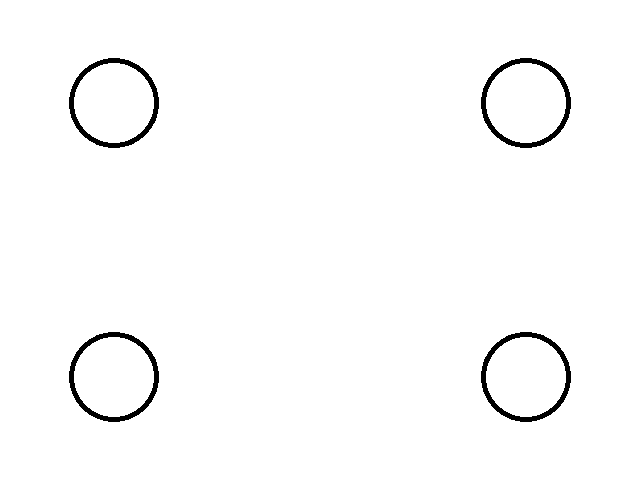
\includegraphics[width=0.5\textwidth]{figures/fsm.png}
\caption{Finite State Machine for Hand Selection States}
\label{fig:fsm}
\end{figure}
Holograsp currently has two Layer-2 input processing classes. The first examines finger coordinates to distinguish poses based
on the index finger and the thumb; the point of interest (used for a cursor or a selection point) would be the midpoint of the tip
of the thumb and the tip of the index finger, and different states were triggered based on whether the two fingers were pinched
together or were separate. This was accomplished via a simple finite state machine illustrated in Figure~\ref{fig:fsm}. We also
applied hysteresis to the state transitions to account for tracking noise; 5 consecutive frames indicating the same state transition
were necessary before a state transition occured.

The second Layer-2 class has a simpler and tends to be more robust. The mechanism simply selects the closest blob of pixels to the monitor
as the point of interest. For speed and simplicity, the default algorithm looks at neighborhoods of nine pixels to determine the closest blob of pixels,
and takes the average of the corresponding points in space to be the point of interest. This mechanism also applies some simple filtering to
smooth each coordinate of the resulting point, since this input method was subject to varying amounts of jitter. Several simple
smoothing methods can be used; we found a double moving average filter with a window size of 5 to be appropriate for the data rates of
our input devices. Many filters are included in Holograsp's implementation, mostly adapted from \cite{brown2004smoothing}. This class was
used in the experiment application because of its robustness.

\subsection{Calibration of Coordinate Systems}
As Holograsp involves a spatially accurate input and output systems, there are two distinct calibration steps needed. The calibration
of camera coordinates with world coordinates is a well-understood problem in computer vision and augmented reality.
However, it is much harder to calibrate the stereoscopic display space given the limitations of the 3D Vision Automatic
system, and more approximate methods must be used.
\subsubsection{Camera to World Calibration}$ $\\
To convert camera coordinates into world coordinates, we used the simple fiducial marker tracker included in the ARToolkit software
library \footnote{http://www.hitl.washington.edu/artoolkit/}, first introduced in \cite{artoolkit}. This determines the camera's position
and orientation in the form of a matrix $M_{RT}$ mapping homogeneous coordinates in world space to camera space.

\begin{figure}
\centering

\includegraphics[width=0.5\textwidth]{figures/hiro.png}
\caption{Fiducial Marker used in ARToolkit}
\label{fig:hiro}
\end{figure}

Camera calibration using fiducial markers is very well understood and is a fundamental part of most augmented reality applications. Fiducial
markers, such as the one depicted in Figure~\ref{fig:hiro}, are generally composed of a thick black border and an inner area
containing distinguishing features. The standard algorithm first thresholds the camera frame and looks for regions that are composed of four straight lines.
This yields the equations of two perpendicular line segments, as projected onto the camera plane. Using the perspective projection equation
for the camera, which depends only on the camera's field of view and aspect ratio, the algorithm can compute the plane containing two
parallel line segments. This plane determines the camera's orientation with respect to the marker. The translation of the camera can then be
easily obtained by substituting the coordinates of the fiducial marker corners into the projection equation. This algorithm is described in
detail in \cite{kato1999marker}.
\subsubsection{Stereoscopic Display to World Calibration}$ $\\
The major benefit of using a stereoscopic 3D monitor instead of a head-mounted display is that the 3D calibration is less sensitive to
head movements when using the monitor. We operated under the assumption that the user would be approximately 80cm away from the monitor
and the neutral eye position would be directed at the middle of the monitor. We also provide users with a mechanism to fine tune the
calibration, since we could not guarantee identical head positioning each time the system was used.

We formulated the display coordinate to world coordinate calibration as a linear transformation.

$$M_{d} = \left(
\begin{array}{cccc}
a & 0 & a_z & a_t \\
0 & b & b_z & b_t \\
0 & 0 & c_z & c_t \\
0 & 0 &   0 &   1
\end{array}\right)$$

This matrix is considerably simpler than a full rotation-translation matrix. This simplification was based on several assumptions:
\begin{itemize}
\item True stereoscopic rendering, using quad-buffered stereo, requires the location and orientation of the viewer and the eye separation.
Camera intrinsic, perspective, and transformation matrices are all linear, as is the stereoscopic approximation used in Nvidia 3D Vision
Automatic. in particular, the $c$ depth convergence parameter is simply an artificial depth offset. We therefore felt justified in choosing
a linear transformation to represent the display to world calibration matrix.
\item Nvidia 3D Vision Automatic does not allow for head roll; this is a fairly safe operating assumption since people generally do
not tilt their heads to the side significantly when working with visual displays. Thus, we assume that the $x$ and $y$ coordinates are
independent. This makes the process of obtaining measurements much simpler, since we can indepently calibrate the $x$ and $y$ dimensions.
\item We also assume that objects at a constant distance from the monitor will have the same $z$ coordinate, regardless
of position on the monitor. This relies on the assumption that the user is approximately centered with respect to the monitor. This is
a safe assumption because it is fairly straightforward for the user to tell if they are severely off-center, and small deviations
do not affect the calibration significantly. Therefore, the $z$ coordinate is independent of the $x$ and $y$ coordinates.
\item $a_z, b_z$ are necessary because the display space is actually a frustrum; the base of the frustrum is located at the corners of
the monitor, and the apex is at the user's head. Therefore the distance from the monitor affects the world $x,y$ coordinates at a given
pixel; for example, for an object near the top of the monitor, moving further away from the display makes the apparent world coordinates of the
object closer to the center of the display.
\end{itemize}

Initial estimates for these values were obtained by displaying models with very clear depth cues at the center of the screen at ten screen $z$ depths,
with screen coordinates $(0,0,z)$. The apparent location of the model in world coordinates, $(x_w, y_w, z_w)$, was measured by hand. This gave the following equations
$$a_zz + a_t = x_w$$
$$b_zz + b_t = y_w$$
$$c_zz + c_t = z_w$$
We then performed a linear regression on each coordinate to obtain $a_z, a_t, b_z, b_t, c_z, c_t$.
Then we display the model at ten $z$ depths at the corners of the monitor, with coordinates $(w/2, h/2, z)$ where $w,h$ are the horizontal and vertical
resolution of the monitor, respectively.
$$\frac{aw}{2} + a_zz + a_t = x_w$$
$$\frac{bh}{2} + b_zz + b_t = y_w$$
Linear regressions on the $x$ and $y$ coordinates independently give values for $a,b$ as well as validate our assumption of a linear dependence of $x$ on $z$.

Our fine-tuning calibration was mainly used to adjust the translation parameters $(a_t, b_t, c_t)$. All users during our user study required at least
a small amount of adjustment of these parameters; this was done by eye. We also provided mechanisms to adjust
$(a_z, b_z, c_z)$, since these would change depending on the distance from the monitor. However, we found during our user study that the small range of
head distances and the moderate size of the interaction space meant that adjusting $(a_t, b _t, c_t)$ was sufficient to calibrate points in the
interaction space.

In future iterations of Holograsp, we aim to include an automated calibration workflow. This would involve displaying models at several locations and
having the user indicate gesturally where the objects appeared. We would also like to include at least rudimentary head tracking, involving fiducial
markers or more sophisticated computer vision techniques to recognize heads in depth images.

% ------------------------------------- METHDOLOGY ------------------------------------------
\section{Evaluation Methodology}
Many previous works, such as \cite{study1,mattheiss2011navigating,study2}, have consistently found the
mouse to be faster and more precise for 3D manipulation
tasks than devices with higher degrees of freedom, including in-air devices.
The goal of this experiment was to determine if the poor performance of high DOF devices could
be a result of cognitive separation between the interface and the task to be performed.
\subsection{3D Manipulation Task}
Bowman et. al describe several fundamental tasks in 3D interfaces, primarily selection,
manipulation, navigation, system control, and symbolic input \cite{3dui}. The most fundamental
for many domains are selection and manipulation. For example, in CAD applications or 3D data
analysis, the user often wants to specify a particular point on a virtual object, or a
destination for a new mesh to be created. Traditional methods of selecting a point on an
object generally use "picking", which involves casting a ray from the viewpoint through the
cursor and selecting the nearest point on the object\cite{study1}. However, with a 2 DOF
interface it is extremely difficult to specify an arbitrary point in space; indeed in existing
CAD applications users rely on multiple orthographic projections to decompose coordinates into
several 2D placements \cite{study2}.

Because selecting a point in 3D space is fundamental to many CAD operations, we elected to
evaluate the performance of our novel interface on a placement task, based on the experiments
of \cite{study1, study2}. The placement task involves two objects situated in a 3D space; the
goal of the user is to select a target object and translate it to the position of the
destination object. Various forms of visual feedback are incorporated into this task to
make it more convenient for users; these include orthographic projections, a cursor, color
changes, and other depth cues such as shadows. Alternate evaluation tasks exclude the
translation step, only testing selection \cite{holodesk}, or examining more complex tasks
that involve a rotation as well as a translation (known as "docking") \cite{masliah2000measuring}.

\subsection{Interaction Techniques}
In our experiment we examined two aspects of 3D interaction interfaces: output interfaces and
input interfaces. Our primary interest in investigating output interfaces was whether natural depth cues,
specifically stereoscopy, were better suited to 3D tasks than artificial ones, such as the
standard orthographic projections. In terms of input interfaces, we compare the traditional
mouse interface with a natural user interface that used gesture.

Our goals in comparing both output and input interfaces were based on the belief that the
efficacy of input devices were closely tied to the feedback provided to the user, i.e. the
output methodology. In particular, we hypothesized that natural stereoscopic
depth cues, when spatially coupled with a gestural in-air interface as in Holograsp, would make full use of
physical intuition. With this interface, users could conceive of the task as simply reaching
out to a physical object and moving it to another location with their hands, instead of
indirectly controlling an abstract cursor with their actions.

\subsubsection{Input Interfaces}$ $\\
Both input interfaces involved a cursor element that was controlled by the user's actions. This
element could select and release appropriate virtual objects if the cursor overlapped the object.
However, with the coupled 3D-gesture interface, the cursor could be ignored since it was
calibrated to be at the user's fingertip.

Due to the 2DOF nature of the mouse element, cursor movements were decomposed into two planes.
By default, moving the mouse would move the cursor in the $xy$ plane parallel to the monitor.
The cursor was locked within the screen boundaries. This corresponded to the familiar mouse pointer
manipulation used in the desktop. By holding down the spacebar, the cursor would instead move in the
$xz$ plane, parallel to the table surface. This had an intuitively correspondence to mouse movements; moving
the mouse towards the screen would move the cursor into the screen. The $z$ distance was limited so that the
cursor could not move behind the viewpoint of the scene. The $xz$ motion actually affected the actual $y$-coordinate
in a way that corresponded with the perspective projection. For example, if the cursor near the bottom of the interaction
space, moving the cursor into the screen also moved it downwards in the interaction space; this meant that the screen
coordinates of the cursor would not change with this interaction. An alternate method would have kept the $y$ coordinate
constant during the $xz$ motion, so that the cursor would actually move up or down in screen coordinates as well. However,
we found during preliminary experiments that the perspective-corrected method was much more natural for 2D views, and did
not have a large impact when combined stereoscopic 3D views.

We experimented with two gestural interfaces. The first involved the thumb and index finger of a hand. The cursor would
follow the user's hand when the thumb and index finger were extended and the remaining fingers were curled. The cursor
location was between the thumb and index finger; selection and release were accomplished by pinching the two fingers
together and bringing them apart, respectively. This interface was designed such that moving an object simply felt like
picking it up and dropping it. This interface used the hand pose tracking in the Intel Perceptual Computing SDK.
However, we found that pose recognition
was not robust under arbitrary orientations of the hand with respect to the depth camera. This interfered significantly with
the placement task, since the system would detect false releases fairly often. The closed-source nature of the SDK meant that
we could not modify the tracking algorithms for our setting, either. Thus, for the placement task interface, we elected to
relax the constraint of having a completely gestural interface, instead allowing the use of the keyboard for selection and
deselection. In this simpler interface, the depth camera takes the blob of points nearest to the screen as the cursor location.
The spacebar was the analogue of the left mouse button in the mouse interface, so that the user would hold down the spacebar
to select and move the virtual object, and release the spacebar to release the object. Users would use an extended fingertip as
their pointing tool. This method suffered from occasional problems at extremes of the interaction space (where other parts of the hand
might be closer to the screen than the fingertip), but these did not severely affect task performance.

\subsubsection{Output Interfaces}$ $\\
Both output interfaces incorporated similar feedback elements. Three geometric elements
appeared on the screen: a red icosahedron, representing the object to be manipulated, a
cyan sphere, representing the destination for the icosahedron, and a green tetrahedron,
denoting the cursor. The manipulable icosahedron changed color to blue when the cursor
overlapped it to indicate that it was selectable. When it was selected and was moving
with the cursor, the icosahedron turned green. Similarly, the target sphere turned dark
cyan when the cursor was overlapping it. These feedback elements made the criterion for
performing each action in the task evident -
any movement, selection, or release condition would be clearly indicated to prevent any user
confusion. This is a fundamental user interface design principle \cite{bravenuiworld}.

The output interfaces differed in their presentation of depth cues. In the 2D output mode,
the main view of the screen was a perspective projection of the interaction space that
included an orthographic projection of a top view of the scene to indicate depth. The 3D output mode eliminated the top
view, but rendered the perspective projection in pop-out 3D so that the scene appeared to
float in front of the monitor. The spatial coordinates of the cursor in the full Holograsp interface, when combined
with the stereoscopic view, ensured that there was an exact correspondence between the user's fingertip
and the cursor location. With the 2D display, this spatial correspondence was still present but could not
be aligned with a real-world perception of the world. The indirect correspondence of 2D and in-air interface is the one
often used by novel 3D interaction modes such as the Wiimote in-air interface used in \cite{study1}.

We also experimented with a traditional four-view 2D output
scheme, with top, side, and front orthographic projections in addition to the perspective projection.
This was motivated by the fact that most existing CAD tools use this combination of views as their
primary display modality. However, we found that our conception of the cursor as having its own
3D location conflicted with the primary interaction paradigm of this system. Normally, in CAD programs
the cursor is tied to a single view at any time; the particular plane of interaction depends on which view
the cursor is in. In contrast, conceiving of the cursor as a scene element with its own 3D location means
that the cursor is located in all of the views. This was confusing to our preliminary testers, who did not
have extensive 3D modelling experience; thus we elected to keep the intuitive perspective view as the
main display and rely on a smaller top projection reminiscent of the "minimap" projection used in many
video games to convey depth information.

% ------------------------------------- USER STUDY ----------------------------------------
\section{User Study}
\subsection{Procedure}
The user study was centered around the 3D placement task. Volunteers were solicited by
through word of mouth and departmental Facebook groups. We collected data from 14 participants,
consisting of 13 males and one female. One male participant was a graduate student in computer
science; 10 participants were undergraduates in computer science and the remaining participants
concentrated in East Asian Studies, Mathematics, and Astrophysics.

Before the task participants were asked to fill out a survey describing their experience with
gestural systems, stereoscopic 3D, CAD and 3D modelling, and video gaming.

The participants were then introduced to the system to familiarize themselves with the placement task, the pop-out
stereoscopy and the gesture system. An experimenter was with the participant at all times during
the use of the system. The participants were first exposed to the pop-out stereoscopic effects;
if they had trouble perceiving the objects they were given an explanation of how the stereoscopy
worked and some simple eye exercises to try. Then they were reintroduced to the stereoscopic effects
at a slightly less intense level where objects appeared closer to the screen, and they were encouraged
to interact with the system using the mouse interface. All participants were then introduced to the placement
task using the 3D-mouse interface and encouraged to finish five to ten tasks to demonstrate their understanding.
The participant was then introduced to the full Holograsp 3D-gesture interface, including the intuition behind the aligned gesture and display
spaces and the calibration procedure. They once again had the opportunity to finish up to ten tasks using this interface.

After familiarizing themselves with the interface, the participants then performed the full round of timing experiments. These
experiments used a within-subjects design, with independent variables of output modality (2D vs. 3D) and input modality (gesture vs. mouse).
For each of the four interface combinations (2D-Mouse, 2D-Gesture, 3D-Mouse, and 3D-Gesture), the participant completed a
run of ten consecutive placement tasks. Participants performed two blocks of these 40 tasks, for a total of $(14)(2)(40) = 1120$
placement tasks. Each run of tasks was preceded by one untimed task to give the user time to adapt to the interface, and
in the 3D-Gesture case, perform calibration.

In each task, the locations of the target and destination objects were selected at random in the interaction space. The
ordering of the interfaces within a run was also randomized; the one exception was that the last interface in a block
would not be selected as the first interface in the subsequent block.

The quantitative data collected was the time in milliseconds for every selection and release event. We did not formally
collect data on movement trajectories, but the experimenter did collect qualitative observations on general trends in
trajectories. After completion of the second block, participants were asked to fill out a survey involving several questions
about their perceptions of the interfaces. We asked participants to compare input modalities and output modalities, as well as
make general observations about the efficacy of the system. We also asked a series of short questions asking participants for
the interface choices best fitting a certain criterion, as well as a short justification. These criterion were:
\begin{itemize}
\item Their personal favorite
\item The easiest to use for completing the task
\item The most intuitive
\item The most accurate
\item The one they'd choose if they had to perform the task many times
\item The one they'd recommend to beginners
\end{itemize}
% Error, size, jitter, randomization, trajectories
\subsection{Results}
\begin{figure}
\centering
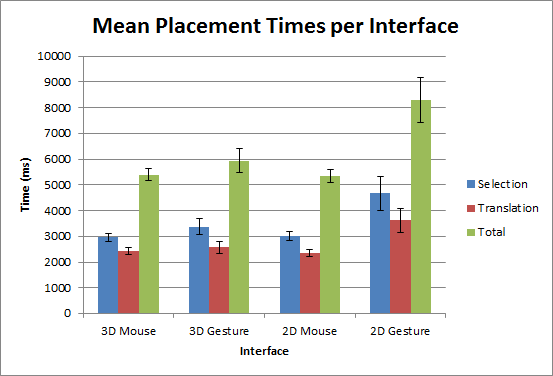
\includegraphics[width=0.7\textwidth]{figures/aggmean.png}
\caption{Mean placement times for each interface in a. time until first
selection, b. time from first selection until task completion, and c. total task
completion time. All data is shown with 95\% confidence intervals.}
\label{fig:aggregate}
\end{figure}
\begin{figure}
\centering
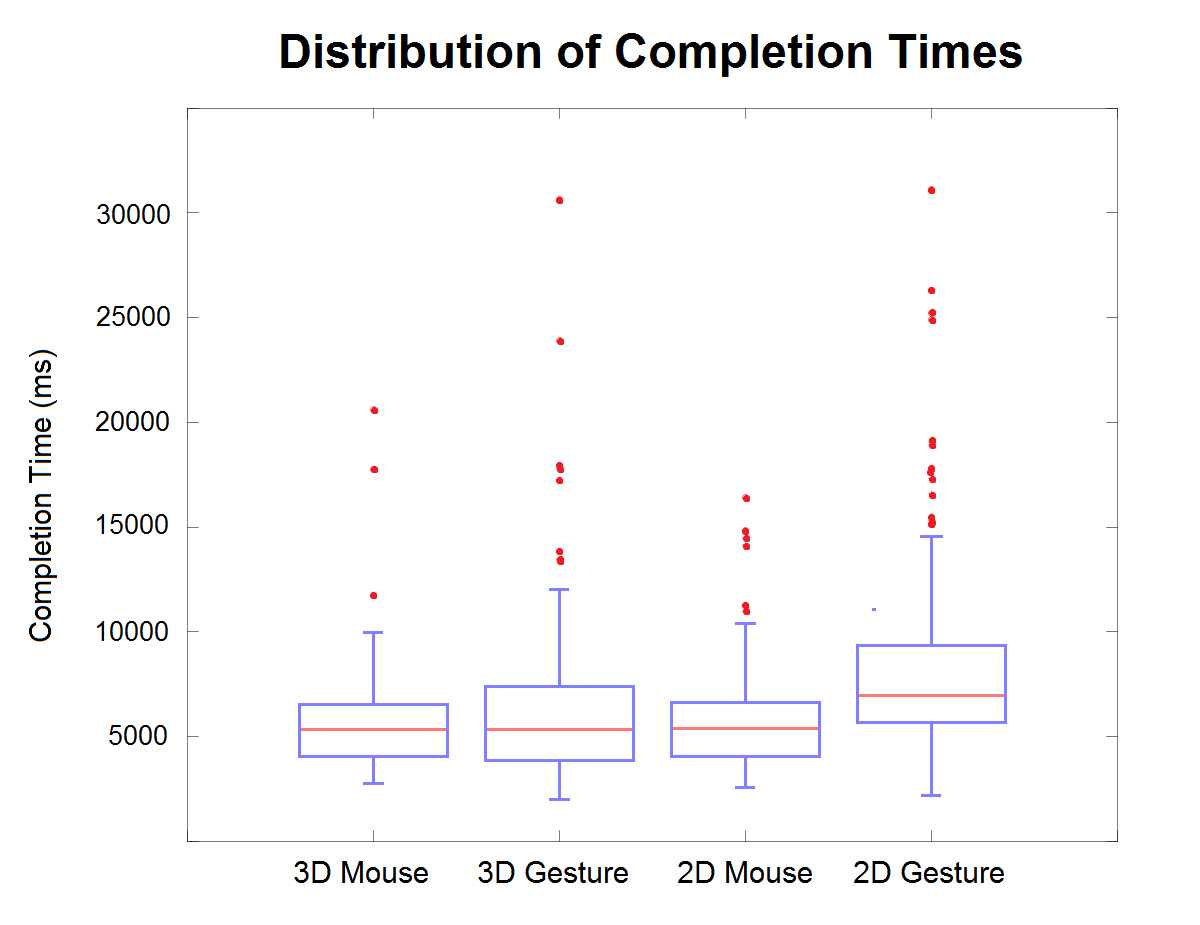
\includegraphics[width=0.7\textwidth]{figures/distribution.png}
\caption{Distribution of total placement times for each interface. Whiskers are
 at most 1.5 IQR in length. Note that three outliers $> 40000$ for the 2D gesture interface are not
shown}
\label{fig:distr}
\end{figure}
Figure~\ref{fig:aggregate} shows the mean times per task for each interface, considering time until first selection, time from first selection until
task completion, and total task completion time. We also show the distribution
of mean placement times in Figure~\ref{fig:distr}. These plots show that the gestural interfaces had more variation in completion times, especially in high completion-time
outliers. Furthermore, a repeated measures ANOVA on the results showed a strong effect of
interface on completion time ($F_{3,39}=7.19, p < 0.001$).
However, no general conclusions can be drawn between the mouse interfaces or the 3D gestural interface; post-hoc analysis showed no significant differences
in mouse interface times ($p > 0.05$) or between the 3D-gesture and either mouse interface ($p > 0.05$). It is clear, however, that the 2D-gesture interface
was worse than the other interfaces ($p < 0.01$).

\begin{figure}
\centering
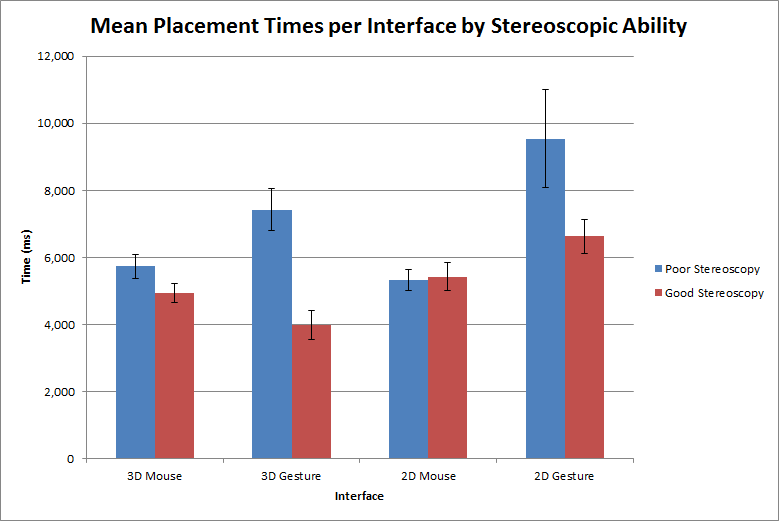
\includegraphics[width=0.7\textwidth]{figures/mean.png}
\caption{Mean placement times for each interface, separated by whether
stereoscopic perception problems were expressed. 95\% confidence intervals are
shown.}
\label{fig:sepmean}
\end{figure}
Because of the lack of conclusive results, we further analyzed post-hoc the results for each individual participant. This data revealed several more interesting observations.
The most significant observation was that most people were either significantly faster with both mouse interfaces, or significantly faster with the 3D-Gesture interface.
This contrasts with the aggregated data, which would suggest that each participant would have similar completion times between the mouse interfaces and the 3D-gesture
interface. Inspection of survey results revealed that the critical distinction
was whether participants had expressed difficulty with perceiving
the pop-out stereoscopic effects. Figure~\ref{fig:sepmean} compares the mean
time to task completion for each interface and each stereoscopic perception
group. Pairwise t-tests show significant differences between performance between
the groups for the 3D gesture interface ($p < 0.01$) but not for any other
interfaces ($p > 0.05$).

Because of the large differences in task performance between individuals, we
also examined participant performance relative to their own completion times.
Figure~\ref{fig:mousevs3dg} shows a scatter plot with one point for each
participant. The horizontal component of each point is the participant's mean 3D
mouse time divided by their mean 3D gesture time; likewise the vertical
component of each plot is the participant's mean 2D mouse time divided by their
mean 3D gesture time.  A similar plot is shown in Figure~\ref{fig:gesturevs2dm},
which compares mean completion times of the two gestural interfaces normalized
by the 2D mouse mean completion time.

\begin{figure}[h]
\centering
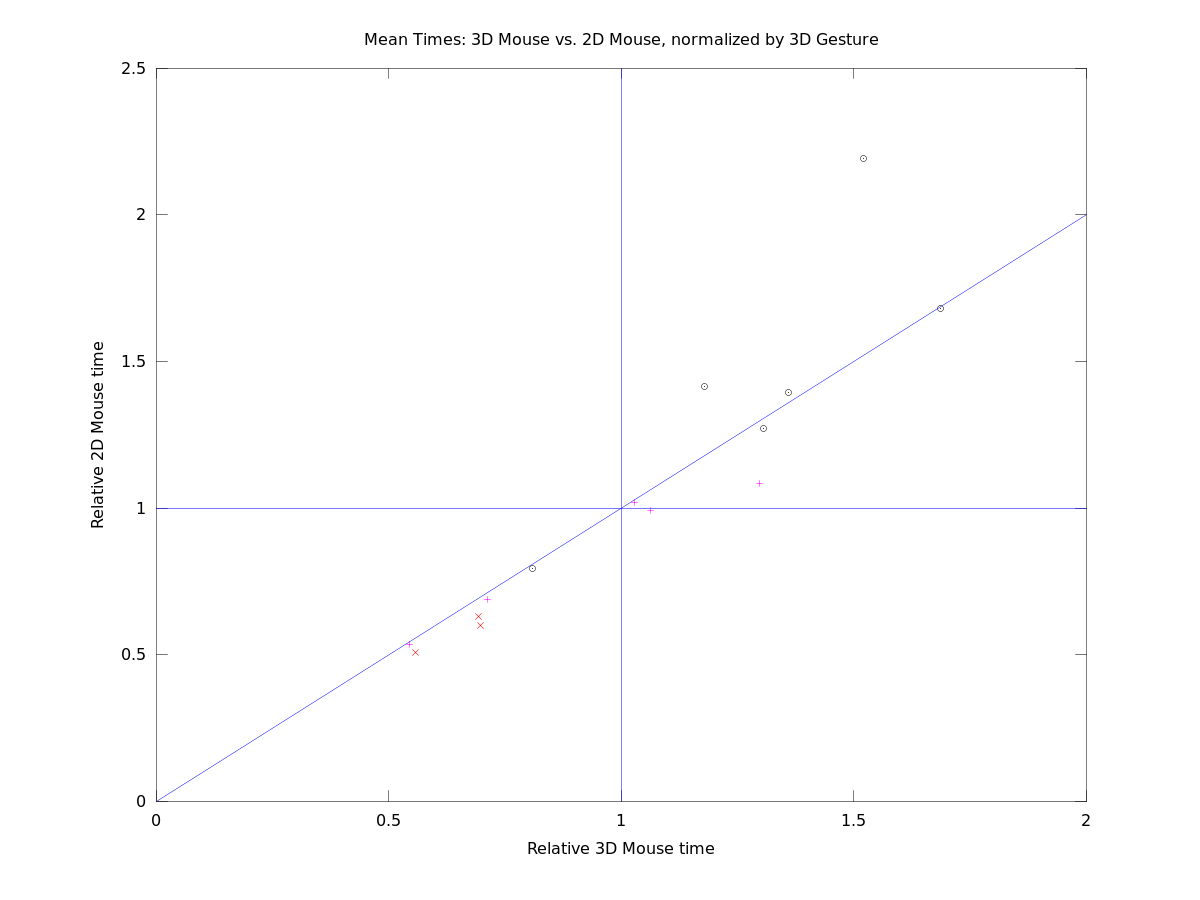
\includegraphics[width=0.7\textwidth]{figures/mousebygesture3d.png}
\caption{Relative completion times for 3D mouse and 2D mouse interfaces,
normalized by 3D gesture completion times. \\
Legend: Red x denotes severe problems with stereoscopic perception. Magenta +
denotes occasional problems with stereoscopic perception. Black o denotes no
issues with stereoscopic perception.}
\label{fig:mousevs3dg}
\end{figure}

From Figure~\ref{fig:mousevs3dg}, we can observe that for most participants
the two mouse interfaces were fairly similar in performance, since most points
are fairly close to the $y = x$ line in blue. The plot also shows that the
participants with poor stereoscopic perception tended to be faster with the
mouse interfaces than the gesture interface, since their data points tend to be below
and to the left of the $y = 1, x = 1$ lines. Similarly, participants without
stereoscopic perception issues are above and to the right of $y = 1, x = 1$.

\begin{figure}[h]
\centering
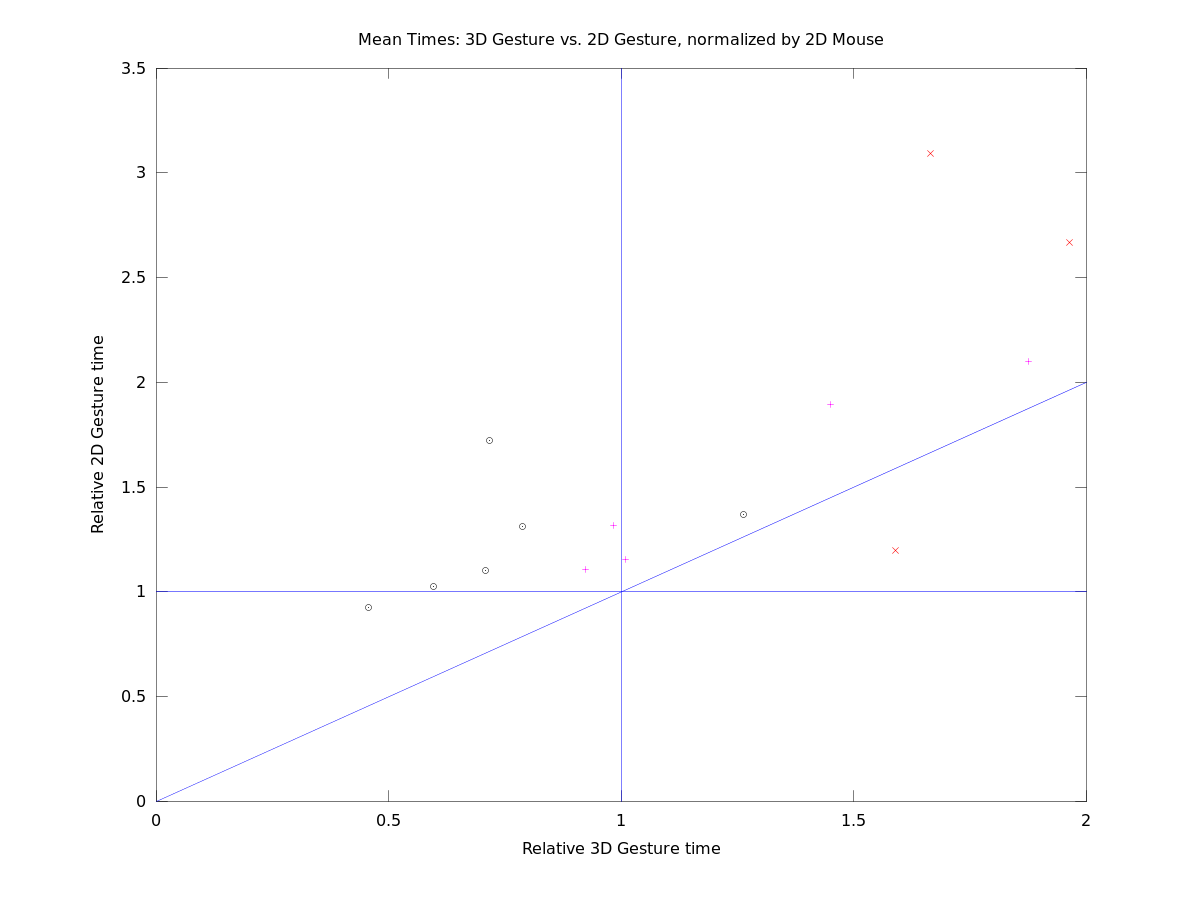
\includegraphics[width=0.7\textwidth]{figures/gesturebymouse2d.png}
\caption{Relative completion times for 3D gesture and 2D gesture interfaces,
normalized by 2D mouse completion times. \\
Legend: Red x denotes severe problems with stereoscopic perception. Magenta +
denotes occasional problems with stereoscopic perception. Black o denotes no
issues with stereoscopic perception.}
\label{fig:gesturevs2dm}
\end{figure}
From Figure~\ref{fig:gesturevs2dm}, we can see that almost all participants were
faster with the 3D gestural interface than the 2D gestural interface (most
points are above $y = x$). Likewise, almost all participants are better with the
2D mouse interface than the 2D gesture interface (most points are above $y=1$).
Finally, we note once again that the participants with good stereoscopic
perception ability tend to have faster 3D gesture times than 2D mouse times (to
the left of $x=1$) and those with poor stereoscopic perception were faster with
the 2D mouse than the 2D gesture.

\begin{figure}[h]
\centering
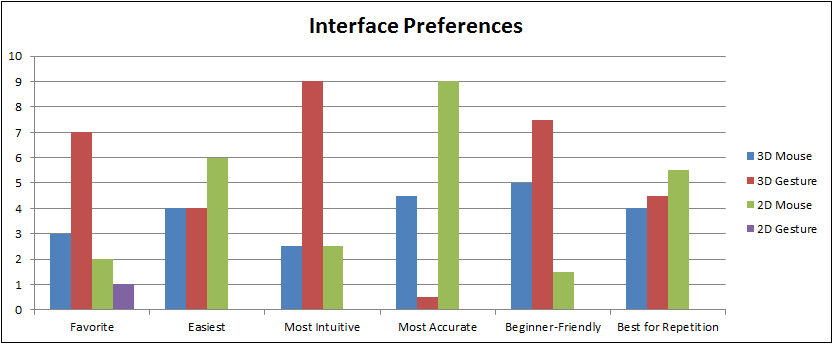
\includegraphics[width=0.8\textwidth]{figures/survey.png}
\caption{Interface preferences for post-experiment survey}
\label{fig:survey}
\end{figure}
The results of the survey for the interface preference questions are shown in
Figure~\ref{fig:survey}.

% ------------------------------------- DISCUSSION ----------------------------------------
\section{Discussion}
In general, no conclusive evidence was found to suggest Holograsp was significantly better than existing interfaces. The difference in mean
completion times were not significant between the Holograsp interface and mouse interfaces (whether stereoscopic or 2D). However, some very
interesting results appear when we take stereoscopic perception into account. When we examine participants who expressed no difficulty with
stereoscopic perception, the Holograsp interface was far and away the best interface. In fact the four fastest mean completion times were
performed with Holograsp. This supports our initial theory that aligned gesture and display space was beneficial to performance, since weak
stereoscopic perception implies that lack of a true display volume. However, this analysis is not conclusive, especially since these conclusions
were drawn post-hoc. It is possible, for instance, that participants wished to justify poor performance by drawing attention to stereoscopic issues.
We also note that those who did not express issues with stereoscopy on average performed better than their counterparts for all interfaces, suggesting
that spatial reasoning skills may be correlated with stereoscopic perception ability.

In future studies, the most important goal would be to formally
control for stereoscopic perception, since this seemed to be the missing factor in our hypotheses. The best way to do this
would be to provide an objective test of stereoscopic ability before the timed task evaluation. We also
would like to investigate the effects of learning as well as fatigue by holding longer experiments with
more blocks per person. One other common factor that we did not examine was accuracy; for example in \cite{study1}
both speed and accuracy were measured. However, analyzing speed and accuracy independently is difficult because
there is a natural speed/accuracy tradeoff. It is hard to specify to participants an appropriate level of speed
or accuracy desired. One method commonly used in HCI is Fitts' Law, which gives an explicit relationship between
speed and accuracy. However, Fitts' Law was formulated for one-dimensional tasks and no generally accepted extension
to higher dimensions has been found (but see \cite{mackenzie1992extending, monk1985fitts, murata2001extending} for some analyses of Fitts-like equations for higher
dimensional interaction tasks). 

It is interesting to note that no significant difference was found between the two mouse interfaces. In particular, we also
considered whether the visual feedback and task might be biased for or against a specific interface combination. For example, the
complexity of the scene would easily affect the required accuracy for a placement task; similarly the multiview 2D display interface
encourages the conceptualization of the task as two separate placements. We found the results of \cite{study2} especially intriguing,
since the addition of one new feedback element was enough to completely change results on the same task. This suggests that the details
of visual feedback are as important, if not more important, than the actual input modality; it also means that applications must be
designed very carefully, rather than using generic interface patterns. Applications also are reasonably far removed from the simple tasks
of repeated placement, and thus we would like to compare Holograsp to traditional interfaces for actual 3D design tasks, rather than abstractions
of these tasks. Even with task abstractions, we are interested in testing different tasks, such as rotation or docking, and compare Holograsp's
performance with traditional interfaces.

One very illuminating observation was the trajectories that participants took to move the target object.
For mouse interfaces, it was fairly universal to position the shape on one plane, and then move it in only one dimension on the other
plane to its final destination. For example, in the perspective view, they would overlap the image of the icosahedron and the sphere ($xy$
alignment) and then adjust the $z$ coordinate according to depth cues. This was naturally encouraged by the decomposition of the mouse interface into two separate
modes. Surprisingly, many participants adopted the same tactic for the gestural interfaces as well, especially those with weaker stereoscopic
perception. This was perhaps the major difference between the trajectories of the two stereoscopic perception ability groups. 
Whereas those with strong stereoscopic perception would take a direct path, those with
weaker stereoscopic perception would overlap the images in $xy$ and then reach forward or backwards until the $z$ matched, just as with the mouse
interfaces. Quantitative analyses of movement trajectories are rare but not absent from the literature (see \cite{integralityseparability}), however
several works such as \cite{kruijff2006unconventional} visualize and qualitatively analyze trajectories. More formal quantitative trajectory analysis 
would be a fruitful area of investigation for future 3D interfaces.

It was evident from survey comments that technical details in the Holograsp interface also require significant
polishing. Ten of the participants explicitly mentioned jitter as a problem with the gestural interface. We anticipate
that using better algorithms and more accurate sensors, such as the Leap, will greatly enhance the usability of the
gestural interface. Surprisingly, no users commented on stereoscopic inconsistencies caused by occlusions. We expected
occlusion to be a significant downside to using a 3D monitor, since it was not possible to display a virtual object in front
of a user's finger if the object was virtually located in front of the finger. This likely was a result of the sparse 3D
scene and the simple manipulations involved in the study. We did have two users comment that calibration
was noticeably affected when they moved their heads. This suggests that head and viewpoint tracking would greatly enhance the 
realism of the virtual scene.

% ------------------------------------- CONCLUSION ----------------------------------------
\section{Conclusion}
In this paper, we presented the Holograsp system. Holograsp provides a natural way to interact with 3D data by colocating gestural interaction
space with a stereoscopic display volume. Holograsp knows that, if you place your finger on a virtual object, then you are interacting with that object at
that point. With this sytem, we allow natural interactions such as grabbing a virtual object as if it were a real one.

We also evaluated the Holograsp system by comparing it to traditional input and output systems. We performed a user study to determine whether
using Holograsp was faster than other interfaces in a 3D placement task. We separated this analysis into two axes: Holograsp's 3D stereoscopic
versus traditional multiview 2D displays with orthographic projections, and the gestural in-air interface versus traditional mouse inputs. We
found that, for users who could perceive the colocated stereoscopic display, Holograsp was significantly faster than any other interface combination;
however many users who did experience difficulties with stereoscopic perception, mouse interfaces were noticeably faster than gestural interfaces.
This investigation showed promising results as a pilot study, but more experimentation is needed to provide conclusive support for these interfaces.

Despite the shortcomings of the current system, the possibilities presented by Holograsp are quite exciting. Holograsp provides a framework that
can support a full 3D modelling application with intuitive manipulation input mappings. The computer systems depicted in the Iron Man films are
an especially compelling example of where this could lead, showing possibilities for natural interaction with 3D CAD in the design of machinery
and suits, and 3D data analysis in the manipulation of maps and graphs. We aim to allow the user to treat the virtual world as part of the real
world, and Holograsp shows great promise in fulfilling this vision.

\newpage
\bstctlcite{bstctl:etal, bstctl:nodash, bstctl:simpurl}
\bibliographystyle{IEEEtranS}
\bibliography{references}

\end{document}
